% GENERATED BY build.py FROM cv.json — DO NOT EDIT THIS FILE DIRECTLY.
% ============================================================
%  Taehyun Nam — Curriculum Vitae
%  Compile:  pdflatex cv.tex   (twice, for correct page refs)
%  Needs:    assets/photo.jpg
% ============================================================
\documentclass[11pt,a4paper]{article}

\usepackage[T1]{fontenc}
\usepackage[utf8]{inputenc}
\usepackage{mathptmx}                     % Times text
\usepackage[margin=1in,top=0.9in,bottom=0.9in]{geometry}
\usepackage{graphicx}
\usepackage{enumitem}
\usepackage{xcolor}
\usepackage{ragged2e}
\usepackage[hidelinks]{hyperref}
\usepackage{xurl}                         % allow long DOIs to break across lines
\usepackage{fancyhdr}
\setlength{\emergencystretch}{3em}

\hypersetup{
  pdftitle={Taehyun Nam — Curriculum Vitae},
  pdfauthor={Taehyun Nam},
  colorlinks=true, linkcolor=black, urlcolor=black, citecolor=black
}

% ---- spacing ------------------------------------------------
\setlength{\parindent}{0pt}
\setlength{\parskip}{0pt}
\linespread{1.06}
\pagestyle{fancy}
\fancyhf{}
\renewcommand{\headrulewidth}{0pt}
\fancyfoot[R]{\footnotesize Taehyun Nam \textperiodcentered\ \thepage}

% ---- building blocks ----------------------------------------
% Section heading: bold + underlined, as in the original document
\newcommand{\cvsection}[1]{%
  \vspace{10pt}%
  {\bfseries\underline{#1}}\par
  \vspace{4pt}%
}

% Two-column entry: left = date/label, right = content
\newlength{\leftcol}\setlength{\leftcol}{1.75in}
\newlength{\rightcol}
\setlength{\rightcol}{\dimexpr\textwidth-\leftcol-6pt\relax}
\newcommand{\entry}[2]{%
  \begin{minipage}[t]{\leftcol}\RaggedRight #1\end{minipage}\hspace{6pt}%
  \begin{minipage}[t]{\rightcol}\RaggedRight #2\end{minipage}\par
  \vspace{5pt}%
}

% Narrow label column for personal details
\newcommand{\field}[2]{%
  \begin{minipage}[t]{1.05in}#1\end{minipage}%
  \begin{minipage}[t]{\dimexpr\textwidth-1.05in\relax}#2\end{minipage}\par
  \vspace{2pt}%
}

\newcommand{\me}[1]{\underline{\textbf{#1}}}
\newcommand{\dg}{\textsuperscript{\dag}}
\newcommand{\venue}[1]{\textit{#1}}

\setlist[itemize]{leftmargin=1.4em,topsep=2pt,itemsep=1pt,parsep=0pt,label=\textbullet}
\setlist[enumerate]{leftmargin=1.6em,topsep=2pt,itemsep=4pt,parsep=0pt}

% ============================================================
\begin{document}

% ---- header -------------------------------------------------
\begin{minipage}[t]{\dimexpr\textwidth-1.25in\relax}
  \vspace{0pt}
  {\LARGE\bfseries Curriculum Vitae}\par
  \vspace{16pt}
  {\bfseries\underline{Personal details}}\par
  \vspace{5pt}
  \field{Name}{Taehyun Nam}
  \field{Mobile}{+82-42-350-3976}
  \field{Email}{\href{mailto:taehyun.nam@kaist.ac.kr}{taehyun.nam@kaist.ac.kr}}
  \field{Date of Birth}{2001.04.19.}
  \field{Address}{291 Daehak-ro, Yuseong-gu, Daejeon, Republic of Korea}
  \field{Links}{\href{https://scholar.google.com/citations?user=gRV3-qYAAAAJ}{Google Scholar}
        \;\textperiodcentered\;
        \href{https://orcid.org/0009-0005-3489-1133}{ORCID 0009-0005-3489-1133}
        \;\textperiodcentered\;
        \href{https://www.linkedin.com/in/nth0419/}{LinkedIn}}
\end{minipage}\hfill
\begin{minipage}[t]{1.1in}
  \vspace{0pt}
  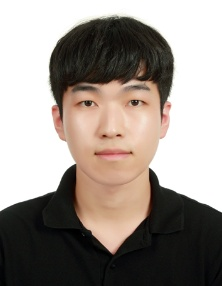
\includegraphics[width=1.01in,height=1.3in]{assets/photo.jpg}
\end{minipage}

\cvsection{Personal Statement}
I am a Ph.D. student in Chemical and Biomolecular Engineering at KAIST, pursuing \textit{material- and process-level engineering} of organic and inorganic semiconductors, and their device-level applications in neuromorphic systems, with a particular focus on \textit{initiated Chemical Vapor Deposition (iCVD)}.

\cvsection{Academic Education}
\entry{Mar 2025 – Current}{Ph.D., Dept. of Chemical and Biomolecular Engineering at KAIST\\
  GPA: 4.03/4.3\\
  Advisor: Prof. Sung Gap Im}
\entry{Mar 2023 – Feb 2025}{M.S., Dept. of Chemical and Biomolecular Engineering at KAIST\\
  GPA: 4.03/4.3\\
  Advisor: Prof. Sung Gap Im}
\entry{Mar 2019 – Feb 2023}{B.S., Dept. of Chemical Engineering at Pohang University of Science and Technology (POSTECH)\\
  GPA: 4.06/4.3 (Summa Cum Laude)}

\cvsection{Work Experiences}
\entry{May 2026 – Nov 2026}{Visiting Scholar, Dept. of Materials Science and Engineering at Pennsylvania State University (University Park, Supervisor: Prof. Saptarshi Das)}
\entry{Jul 2022 – Aug 2022}{Intern, LOTTE Chemical Intellectual Properties Strategy Team}
\entry{Jan 2022 – Feb 2022}{Intern, Korea Advanced Institute of Science and Technology (KAIST), Functional Thin Film Laboratory (Supervisor: Prof. Sung Gap Im)}
\entry{Sep 2021 – Dec 2021}{Intern, Pohang University of Science and Technology (POSTECH), Chemical Engineering Lab (Supervisor: Prof. Won Bae Kim)}
\entry{Jun 2021 – Aug 2021}{Intern, SK Hynix Future Technology R\&D Center NAND Etch Team}

\cvsection{Honors and Awards}
\entry{Mar 2023 – Current}{KAIST Government Scholarship (Full tuition)}
\entry{Mar 2021 – Feb 2023}{National Science \& Technology Scholarship, Korea Student Aid Foundation (Full tuition, merit-based scholarship)}
\entry{Mar 2019 – Feb 2021}{Jigok Scholarship, POSTECH (Full tuition for 4 semesters)}

\cvsection{Research Area}
\textbf{1. Development of p-type tellurium-based electronic devices}\par
\vspace{3pt}
\hspace{1.2em}a) High-hole-mobility p-type tellurium thin-film transistors enabled by iCVD-based polymeric passivation layers
\begin{itemize}
  \item Exploration and optimization of polymeric passivation layers to enhance switching characteristics of p-type transistor devices, including on/off ratio, carrier mobility, and threshold voltage
  \item Analysis of carrier transport mechanisms through spectroscopic techniques (e.g., UPS, Raman) and electrical characterization (e.g., TLM, Schottky barrier analysis)
  \item Development of vertically integrated CMOS logic circuits and flexible TFTs
\end{itemize}
\vspace{4pt}
\hspace{1.2em}b) Enhancement of contact properties in Te TFTs using thermally decomposable polymeric contact interlayers for an ash-out strategy
\begin{itemize}
  \item Exploration and optimization of polymeric buffer layers to reduce contact resistance and enable higher current levels
  \item Investigation of the ash-out process using in-situ heating-cell ellipsometry
\end{itemize}

\vspace{7pt}
\textbf{2. High-performance vertical organic thin-film transistor devices}\par
\vspace{3pt}
\hspace{1.2em}a) Vertical organic thin-film transistors with vertically aligned carrier transport for high-current and high-frequency operation
\begin{itemize}
  \item Design of unconventional vertical organic thin-film transistor architectures and circuit layouts for complex logic circuits (e.g., ring oscillators, half adders)
  \item Analysis of high-frequency device operation using a fast waveform generator and analyzer module (WGFMU) integrated into the B1500A
\end{itemize}

\vspace{7pt}
\textbf{3. Next-generation neuromorphic devices and their applications}\par
\vspace{3pt}
\hspace{1.2em}a) Gate-injection-type organic synaptic transistors with tunable decay times for reservoir networks targeting human activity recognition
\begin{itemize}
  \item Rational selection and optimization of charge-storage-layer semiconductor materials to modulate gate-induced charge transfer and control EPSC decay characteristics
  \item Implementation of synaptic transistors in various AI and neuromorphic applications (e.g., NeuroSim, machine learning), with a particular focus on human activity recognition tasks using the UCI-HAR dataset
\end{itemize}

\cvsection{Research skills and experiences}
\textbf{Characterization Techniques}
\begin{itemize}
  \item SEM, AFM, FT-IR, XPS · depth profiling, XPS · high-resolution, UPS · depth profiling, Contact angle analyzer, Ellipsometer (optical analysis), XRD, Hall effect measurement
\end{itemize}
\vspace{4pt}
\textbf{Polymer Fabrication \& Surface Engineering}
\begin{itemize}
  \item iCVD-based functional homopolymer and copolymer synthesis, Composition and structure optimization
\end{itemize}
\vspace{4pt}
\textbf{Fabrication and Characterization of Electronic Devices}
\begin{itemize}
  \item 2-terminal devices: MIM, RRAM, 3-terminal devices: TFT, flash memory, synaptic devices, Multi-terminal devices/circuits: inverter, logic gates, ring oscillator, 2D material-based transistor fabrication: sourcing, exfoliation, wet transfer, Device layout designing, Optoelectronic measurement
\end{itemize}
\vspace{4pt}
\textbf{Devices \& Instruments}
\begin{itemize}
  \item iCVD system, Atomic layer deposition (ALD) system, Metal/organic thermal evaporator, E-beam evaporator, E-beam lithography, Photo-lithography mask aligner, Reactive ion etching (RIE) system, Plasma treatment system, Optical microscope, Keysight B1500A semiconductor analyzer, Probe station in glove box with temperature-controlled chuck, Oscilloscope and function generator
\end{itemize}
\vspace{4pt}
\textbf{Software \& Computation}
\begin{itemize}
  \item Python (TensorFlow, Scikit-learn), C, C++, Java, MATLAB, Quantum Espresso, RASPA, ORCA, LAMMPS, OriginLab, ChemDraw, ImageJ, Raith lithography
\end{itemize}
\vspace{4pt}
\textbf{Making \& General}
\begin{itemize}
  \item Fusion360, Cura slicer, Homebrew 3D printer, WordPress, Apache server, MS Office, Linux, Photoshop, Illustrator, Blender
\end{itemize}

\cvsection{Publications (SCIE \& ESCI)}
\begin{enumerate}
  \item \me{Taehyun Nam}\dg, Seung Min Lee\dg, Chungryeol Lee, Changhyeon Lee, Sunwoo Jeong, Seunghwan Seo, Youson Kim, Jeong-ik Park, Seokhyun Hong, Hyung Joong Yun, Kibum Kang, Hocheon Yoo, Junhwan Choi*, and Sung Gap Im*, A High-Hole Mobility Tellurium Transistor with Electron Donating Channel Passivation Layer for Scalable, High-Throughput Electronics, \venue{Advanced Functional Materials}, \textbf{36}, e27125, (2026). \href{https://doi.org/10.1002/adfm.202527125}{doi:10.1002/adfm.202527125}

  \item Youson Kim\dg, \me{Taehyun Nam}\dg, Junyeong Yang, Changsoon Choi, Seun-Bae Jeon* and Sung Gap Im*, Electrolyte–channel interface engineering for STM/LTM differentiation in OECTs for physical reservoir computing, \venue{Nature Communications}, In submission.

  \item Junyeong Yang\dg, Sanghyun Kim\dg, Jeong-Ik Park\dg, Minjeong Kang, Gyuwon Lee, Changmin Lee, \me{Taehyun Nam}, and Sung Gap Im*, Sub-0.3 V Ultra-Low-Voltage Operation of Bilayer RRAM via High-Sulfur Polymer/Inorganic Hybrid Layers for Hardware Synaptic Devices, \venue{Advanced Functional Materials}, In submission.

  \item Chungryeol Lee\dg, Dongho Choi\dg, Sanghoon Park, Jeong-ik Park, \me{Taehyun Nam}, Minjae Jang, Seunghyup Yoo*, and Sung Gap Im*, A light-driven multi-state heterojunction transistor for optoelectronic ternary logic circuits, \venue{Nature Communications}, Accepted, (2026).

  \item Sukwon Jang\dg, Keunho Soh\dg, Chungryeol Lee\dg, \me{Taehyun Nam}, Minjae Jang, Jeong-ik Park, Changhyeon Lee, Junhwan Choi, Jung Ho Yoon*, and Sung Gap Im*, A Unipolar-Driven Synaptic Transistor for Environment-Adaptable Vision System, \venue{Nature Communications}, \textbf{16}, 7636, (2025). \href{https://doi.org/10.1038/s41467-025-63073-2}{doi:10.1038/s41467-025-63073-2}

  \item Sukwon Jang\dg, Youson Kim\dg, Chungryeol Lee\dg, \me{Taehyun Nam}, Jeong-ik Park, Junyeong Yang, Juchan Kim, Bohyun Lee, Sung Gap Im*, Vapor-Phase Deposited Polymer Dielectric Layers for Organic Electronics: Design, Characteristics, and Applications, \venue{Korean Journal of Chemical Engineering}, \textbf{42}, 1931–1949, (2025). \href{https://doi.org/10.1007/s11814-024-00210-5}{doi:10.1007/s11814-024-00210-5}

  \item Jeong-ik Park\dg, Changhyeon Lee\dg, Chungryeol Lee, \me{Taehyun Nam}, Yebin Bak, Sukwon Jang, Hocheon Yoo, Junhwan Choi*, and Sung Gap Im*, Dynamically Reconfigurable Multibit Modulator Enabled by Programmable Anti-Ambipolar Memory Transistors, \venue{Advanced Functional Materials}, In revision.

  \item \me{Taehyun Nam}\dg, Chungryeol Lee\dg, Seokhyun Hong, Jeong-ik Park, Youson Kim, and Sung Gap Im*, Gate-Injection Synaptic Transistor with Tunable Stochastic Memory for Ensemble Reservoir Computing, In preparation.

  \item Seokhyun Hong\dg, \me{Taehyun Nam}\dg, Chungryeol Lee\dg, Jeong-ik Park, Youson Kim, Junhwan Choi* and Sung Gap Im*, High-current Organic Vertical Transistor with Bottom-up Grain Boundary Selective Deposition of Functional Polymeric Layer, In preparation.
\end{enumerate}
\vspace{3pt}
(† These authors contributed equally to this work.  * Corresponding author.)

\cvsection{Conferences and Presentations}
\begin{enumerate}
  \item \me{Taehyun Nam}, Seung Min Lee, Junhwan Choi*, Sung Gap Im*, ``High-Performance p-Type Tellurium Transistor Arrays and Circuits via Vapor Phase Deposited Polymer Passivation'', The 24th International Meeting on Information Display (IMID 2024), August 21, 2024, Jeju, South Korea

  \item \me{Taehyun Nam}, Seung Min Lee, Junhwan Choi*, Sung Gap Im*, ``A High-Hole Mobility Tellurium Transistor with Electron Donating Channel Passivation Layer for Scalable, High-Throughput Electronics'', The 100th Annual Spring Meeting of the Polymer Society of Korea, April 9, 2026, Daejeon, South Korea
\end{enumerate}

\cvsection{Patents}
\begin{enumerate}
  \item Sung Gap Im, \me{Taehyun Nam}, Chungryeol Lee, Sukwon Jang, Sanghoon Ahn, Youngsang Cho, ``Method for film deposition'', (Korea Patent (Priority Claim Country); Application Number: 10-2024-0117056, United States of America Patent; Application Number: 18/921,365).

  \item Youngsang Cho, Sung Gap Im, Yongjin Kim, \me{Taehyun Nam}, Woojin Lee, Chungryeol Lee, Sukwon Jang, ``Method for polymeric layer fabrication'', (Korea Patent; Application Number: 10-2024-0117056).

  \item Sung Gap Im, Sukwon Jang, Chungryeol Lee, \me{Taehyun Nam}, ``Dipole polarization-charge capture synergetic single-polarity driven synapse transistor and artificial sensory system comprising the same'', (Korea Patent; Application Number: 10-2024-0193239, United States of America Patent; Application Number: 19/421,173).

  \item Sung Gap Im, Juchan Kim, Jeong-ik Park, \me{Taehyun Nam}, Bohyun Lee, ``Polymer thin films for semiconductor devices, semiconductor devices comprising the same, and methods for manufacturing semiconductor devices'', (Korean Patent; Application Number: 10-2026-0005661).

  \item Sung Gap Im, \me{Taehyun Nam}, Chungryeol Lee, Minjae Jang, Junyeong Yang, ``Radical initiators for chemical vapor deposition and method for producing polymer thin film using the same'', (Korean Patent; Application Number: 10-2025-0084923).

  \item Sung Gap Im, Wooyoung Chung, \me{Taehyun Nam}, Changmin Lee, ``Sn-based Organic/Inorganic Hybrid UV-sensitive Polymer Thin Film Formed by iCVD Process'', (Korean Patent (Priority Claim Country); In submission, United States of America Patent; In submission).

  \item Sung Gap Im, \me{Taehyun Nam}, Chungryeol Lee, Seokhyun Hong, ``Gate Injection Synaptic Transistor with Tunable Stochastic Memory for Ensemble Reservoir Computing'', (Korean Patent; In submission).
\end{enumerate}

\end{document}
